We will make direction vectors from these line vectors form:

\begin{align}
    \vec{m}_1 = \myvec{-\sqrt{3} & 1}\\
    \vec{m}_2 = \myvec{-1 & \sqrt{3}}
\end{align} 


Now we will find out magnitudes of each vectors $\vec{m}_1$,$\vec{m}_2$ :

\begin{align}
    \norm{\vec{m}_1} = \sqrt{3+1} = 2\\
    \norm{\vec{m}_2} = \sqrt{1+3} = 2
\end{align}

Thus angle between 2 vectors $\vec{m}_1$,$\vec{m}_2$ can be found using dot-product using the formula below,
Let $\theta$ be angle between vectors $\vec{m}_1$,$\vec{m}_2$ then,
\begin{align}
    \theta = \cos^{-1}\brak{{\frac{\vec{m}_1\vec{m}_2^{T}}{\norm{\vec{m_1}}\norm{\vec{m}_2}}}}
\end{align}

By,Putting values into above equation we get,
\begin{align}
    \theta &= \cos^{-1}\brak{\frac{\myvec{-\sqrt{3}&1}\myvec{-1 \\ \sqrt{3}}}{4}} \\
%    \theta &= \cos^{-1}\brak{{\frac{2\times\sqrt{3}}{4}}} \\
 &= \cos^{-1}\brak{{\frac{\sqrt{3}}{2}}}\\
\implies     \theta &= 30\degree
\end{align}

%\begin{figure}[!ht]
%    \centering
%    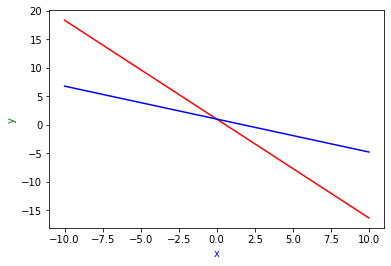
\includegraphics[width=\columnwidth]{Figure_1.png}
%    \caption{Figure}
%% \label{fig: Fig}
%\end{figure}
